\documentclass[11pt,a4paper]{report}
\usepackage[textwidth=37em,vmargin=30mm]{geometry}
\usepackage{calc,xunicode,amsmath,amssymb,paralist,enumitem,tabu,booktabs,datetime2,xeCJK,xeCJKfntef,listings}
\usepackage{tocloft,fancyhdr,tcolorbox,xcolor,graphicx,eso-pic,xltxtra,xelatexemoji}

\newcommand{\envyear}[0]{2025}
\newcommand{\envdatestr}[0]{2025-10-28}
\newcommand{\envfinaldir}[0]{webdb/2025/20251028/final}

\usepackage[hidelinks]{hyperref}
\hypersetup{
    colorlinks=false,
    pdfpagemode=FullScreen,
    pdftitle={Web Digest - \envdatestr}
}

\setlength{\cftbeforechapskip}{10pt}
\renewcommand{\cftchapfont}{\rmfamily\bfseries\large\raggedright}
\setlength{\cftbeforesecskip}{2pt}
\renewcommand{\cftsecfont}{\sffamily\small\raggedright}

\setdefaultleftmargin{2em}{2em}{1em}{1em}{1em}{1em}

\usepackage{xeCJK,xeCJKfntef}
\xeCJKsetup{PunctStyle=plain,RubberPunctSkip=false,CJKglue=\strut\hskip 0pt plus 0.1em minus 0.05em,CJKecglue=\strut\hskip 0.22em plus 0.2em}
\XeTeXlinebreaklocale "zh"
\XeTeXlinebreakskip = 0pt


\setmainfont{Brygada 1918}
\setromanfont{Brygada 1918}
\setsansfont{IBM Plex Sans}
\setmonofont{JetBrains Mono NL}
\setCJKmainfont{Noto Serif CJK SC}
\setCJKromanfont{Noto Serif CJK SC}
\setCJKsansfont{Noto Sans CJK SC}
\setCJKmonofont{Noto Sans CJK SC}

\setlength{\parindent}{0pt}
\setlength{\parskip}{8pt}
\linespread{1.15}

\lstset{
	basicstyle=\ttfamily\footnotesize,
	numbersep=5pt,
	backgroundcolor=\color{black!5},
	showspaces=false,
	showstringspaces=false,
	showtabs=false,
	tabsize=2,
	captionpos=b,
	breaklines=true,
	breakatwhitespace=true,
	breakautoindent=true,
	linewidth=\textwidth
}






\newcommand{\coverpic}[2]{
    % argv: itemurl, authorname
    Cover photo by #2~~(\href{#1}{#1})
}
\newcommand{\makeheader}[0]{
    \begin{titlepage}
        % \newgeometry{hmargin=15mm,tmargin=21mm,bmargin=12mm}
        \begin{center}
            
            \rmfamily\scshape
            \fontspec{BaskervilleF}
            \fontspec{Old Standard}
            \fontsize{59pt}{70pt}\selectfont
            WEB\hfill DIGEST
            
            \vfill
            % \vskip 30pt
            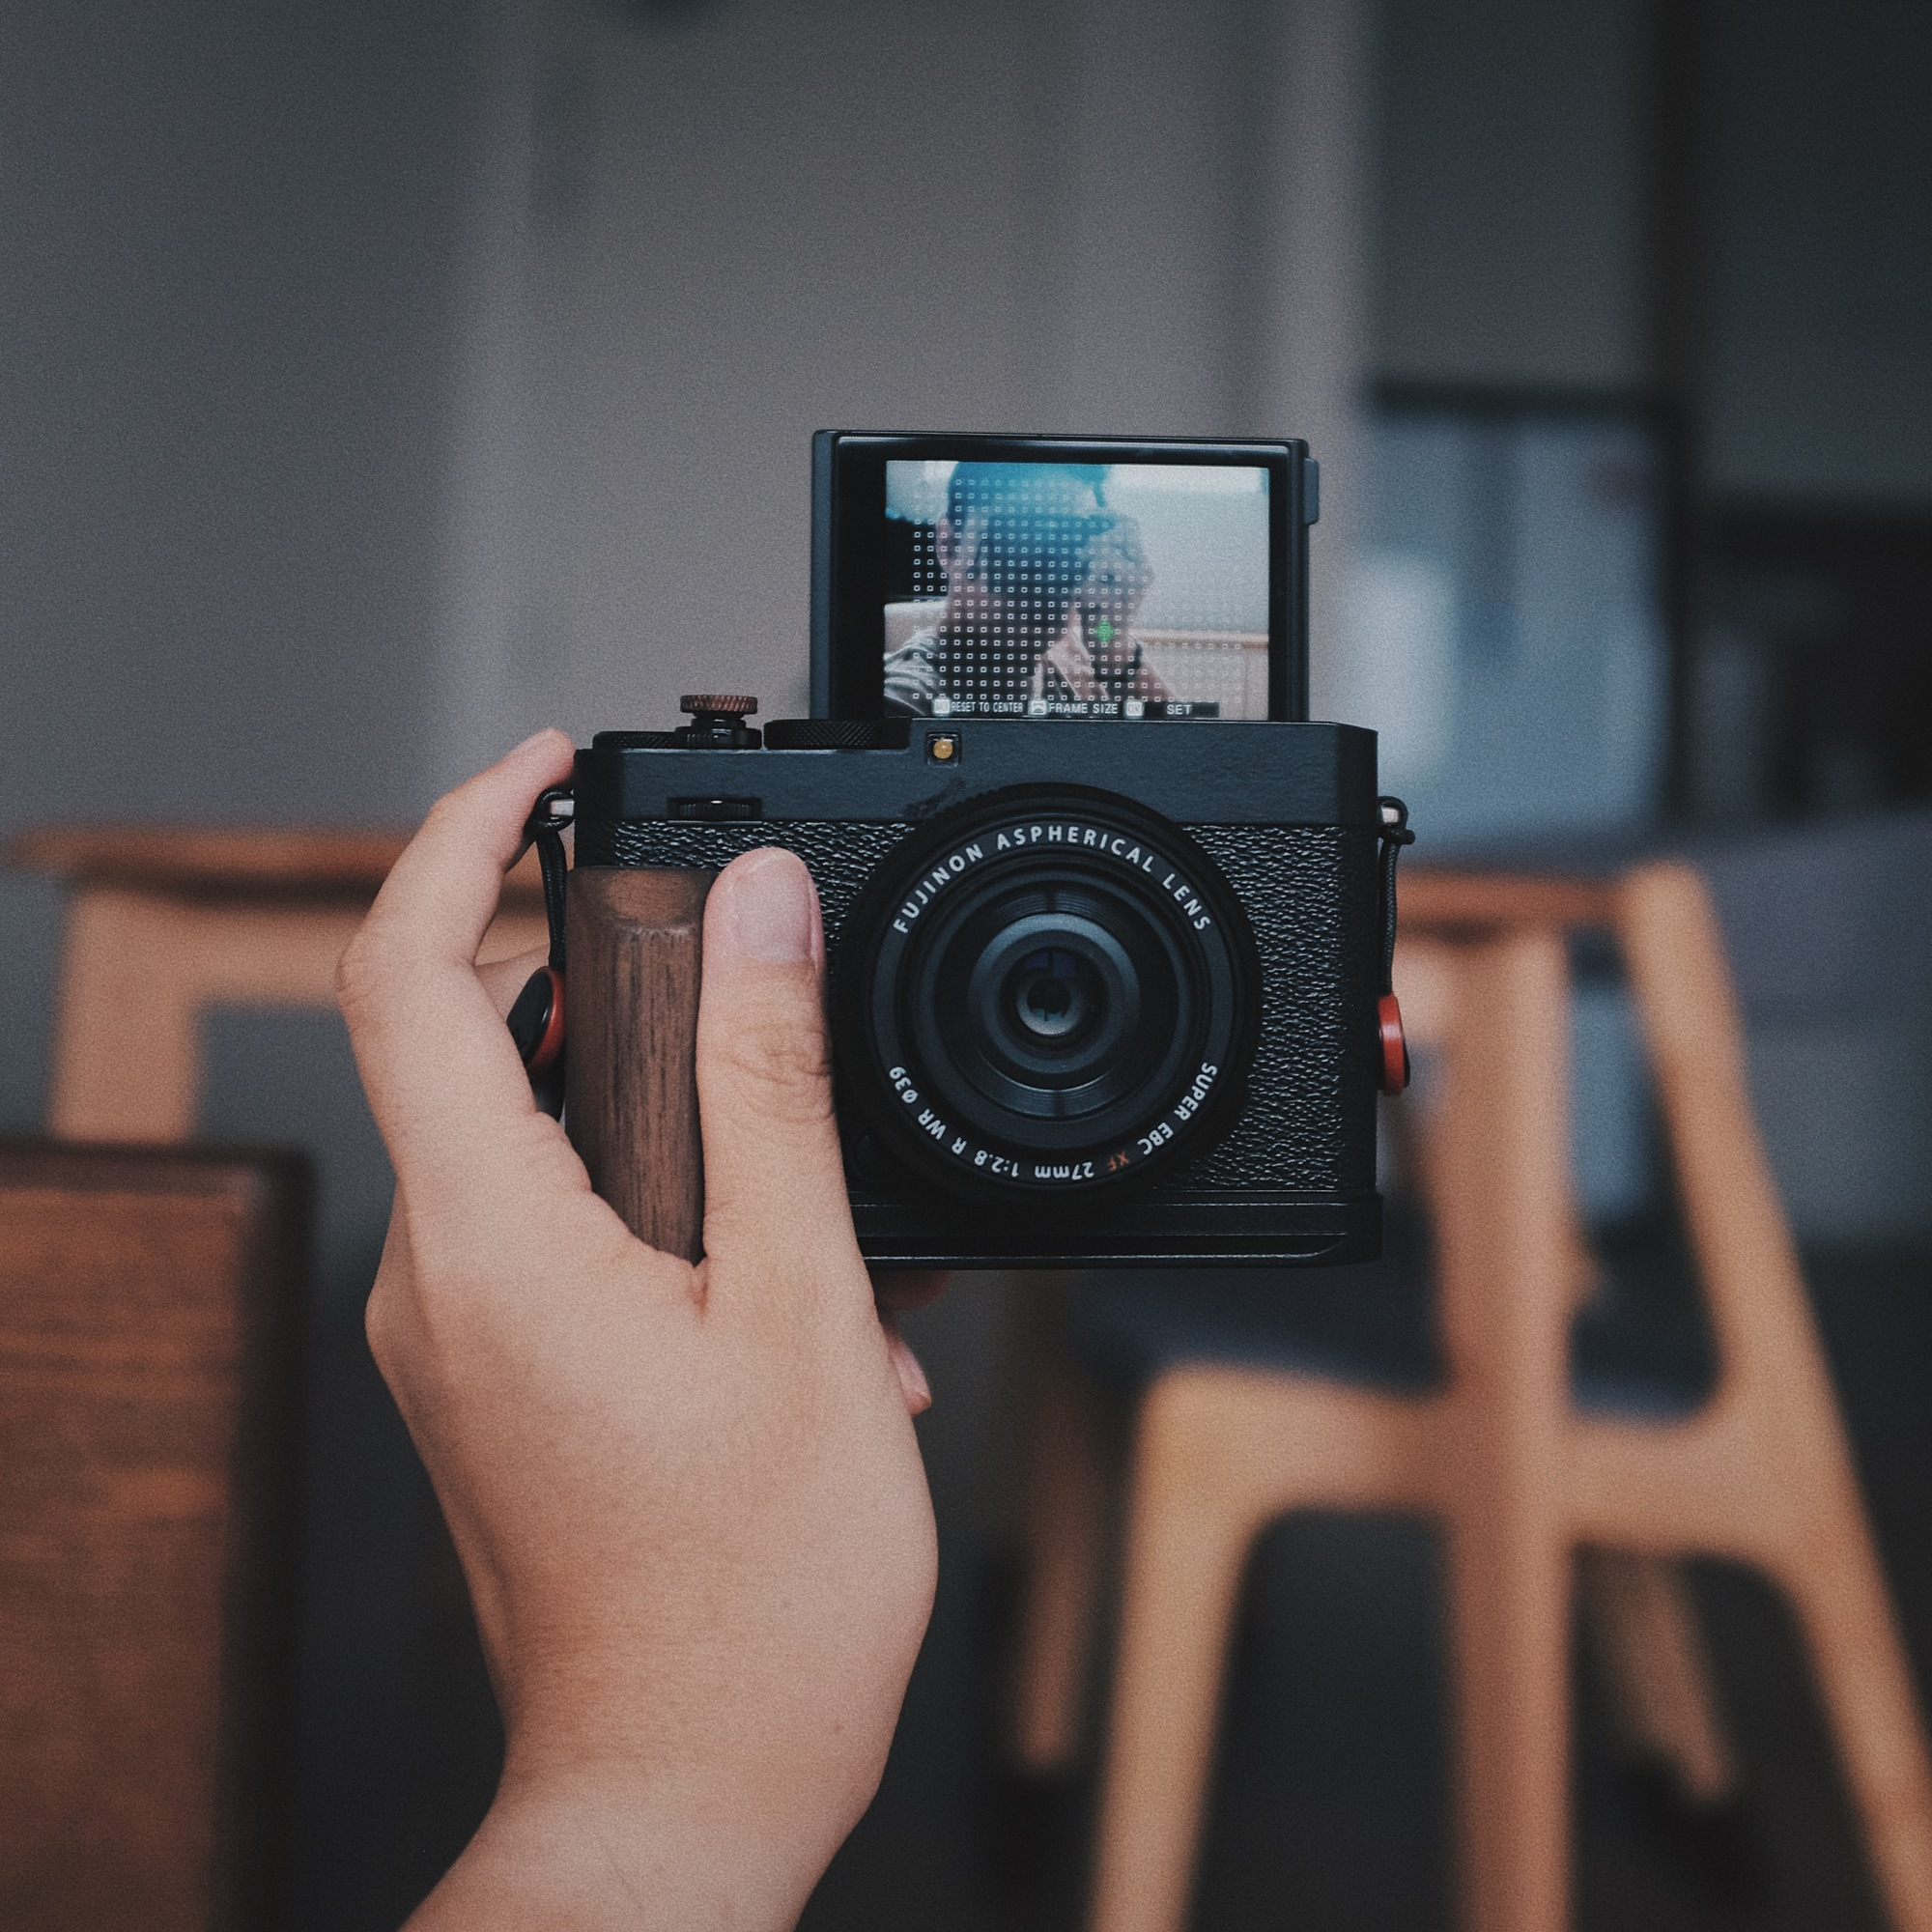
\includegraphics[width=\linewidth]{\envfinaldir/coverpic-prod.jpg}\par
            % \vskip 30pt
            \vfill

            \normalsize\rmfamily\scshape
            \copyright{} The Web Digest Project \hfill\large \envdatestr
        \end{center}
    \end{titlepage}
    % \restoregeometry
}
\newcommand{\simplehref}[1]{%
    \textcolor{blue!80!green}{\href{#1}{#1}}%
}
\renewcommand{\contentsname}{\center\Huge\sffamily\bfseries Contents\par\vskip 20pt}
\newcounter{ipartcounter}
\setcounter{ipartcounter}{0}
\newcommand{\ipart}[1]{
    % \vskip 20pt
    \clearpage
    \stepcounter{ipartcounter}
    \phantomsection
    \addcontentsline{toc}{chapter}{#1}
    % \begin{center}
    %     \Huge
    %     \sffamily\bfseries
    %     #1
    % \end{center}
    % \vskip 20pt plus 7pt
}
\newcounter{ichaptercounter}
\setcounter{ichaptercounter}{0}
\newcommand{\ichapter}[1]{
    % \vskip 20pt
    \clearpage
    \stepcounter{ichaptercounter}
    \phantomsection
    \addcontentsline{toc}{section}{\numberline{\arabic{ichaptercounter}}#1}
    \begin{center}
        \Huge
        \sffamily\bfseries
        #1
    \end{center}
    \vskip 20pt plus 7pt
}
\newcommand{\entrytitlefont}[1]{\subsection*{\raggedright\Large\sffamily\bfseries#1}}
\newcommand{\entryitemGeneric}[2]{
    % argv: title, url
    \parbox{\linewidth}{
        \entrytitlefont{#1}\par\vskip 5pt
        \footnotesize\ttfamily\mdseries
        \simplehref{#2}
    }\vskip 11pt plus 11pt minus 1pt
}
\newcommand{\entryitemGithub}[3]{
    % argv: title, url, desc
    \parbox{\linewidth}{
        \entrytitlefont{#1}\par\vskip 5pt
        \footnotesize\ttfamily\mdseries
        \simplehref{#2}\par\vskip 5pt
        \small\rmfamily\mdseries#3
    }\vskip 11pt plus 11pt minus 1pt
}
\newcommand{\entryitemAp}[3]{
    % argv: title, url, desc
    \parbox{\linewidth}{
        \entrytitlefont{#1}\par\vskip 5pt
        \footnotesize\ttfamily\mdseries
        \simplehref{#2}\par\vskip 5pt
        \small\rmfamily\mdseries#3
    }\vskip 11pt plus 11pt minus 1pt
}
\newcommand{\entryitemHackernews}[3]{
    % argv: title, hnurl, rawurl
    % \parbox{\linewidth}{
    %     \entrytitlefont{#1}\par\vskip 5pt
    %     \footnotesize\ttfamily\mdseries
    %     \simplehref{#3}\par
    %     \textcolor{black!50}{\href{#2}{#2}}
    % }\vskip 11pt plus 11pt minus 1pt
    \begin{minipage}{\linewidth}
            \entrytitlefont{#1}\par\vskip 5pt
            \footnotesize\ttfamily\mdseries
            \simplehref{#3}\par
            \textcolor{black!50}{\href{#2}{#2}}
    \end{minipage}\par\vskip 11pt plus 11pt minus 1pt
}







\begin{document}

\makeheader

\tableofcontents\clearpage




\ipart{Developers}
\ichapter{Hacker News}
\entryitemTwoLinks{Easy RISC-V}{https://news.ycombinator.com/item?id=45726192}{https://dramforever.github.io/easyriscv/}

\entryitemTwoLinks{The PSF has withdrawn a \$1.5M proposal to US Government grant program}{https://news.ycombinator.com/item?id=45726137}{https://simonwillison.net/2025/Oct/27/psf-withdrawn-proposal/}

\entryitemTwoLinks{Amazon targets as many as 30k corporate job cuts, sources say}{https://news.ycombinator.com/item?id=45724813}{https://www.reuters.com/business/world-at-work/amazon-targets-many-30000-corporate-job-cuts-sources-say-2025-10-27/}

\entryitemTwoLinks{Avoid 2:00 and 3:00 am cron jobs (2013)}{https://news.ycombinator.com/item?id=45723554}{https://www.endpointdev.com/blog/2013/04/avoid-200-and-300-am-cron-jobs/}

\entryitemTwoLinks{Why Busy Beaver hunters fear the Antihydra}{https://news.ycombinator.com/item?id=45723359}{https://benbrubaker.com/why-busy-beaver-hunters-fear-the-antihydra/}

\entryitemTwoLinks{JetKVM – Control any computer remotely}{https://news.ycombinator.com/item?id=45723159}{https://jetkvm.com/}

\entryitemTwoLinks{fnox, a secret manager that pairs well with mise}{https://news.ycombinator.com/item?id=45722931}{https://github.com/jdx/mise/discussions/6779}

\entryitemTwoLinks{Claude for Excel}{https://news.ycombinator.com/item?id=45722639}{https://www.claude.com/claude-for-excel}

\entryitemTwoLinks{It's insulting to read AI-generated blog posts}{https://news.ycombinator.com/item?id=45722069}{https://blog.pabloecortez.com/its-insulting-to-read-your-ai-generated-blog-post/}

\entryitemTwoLinks{PSF has withdrawn \$1.5M proposal to US Government grant program}{https://news.ycombinator.com/item?id=45721904}{https://pyfound.blogspot.com/2025/10/NSF-funding-statement.html}

\entryitemTwoLinks{Pyrex catalog from from 1938 with hand-drawn lab glassware [pdf]}{https://news.ycombinator.com/item?id=45721801}{https://exhibitdb.cmog.org/opacimages/Images/Pyrex/Rakow\_1000132877.pdf}

\entryitemTwoLinks{Microsoft in court for allegedly misleading Australians over 365 subscriptions}{https://news.ycombinator.com/item?id=45721682}{https://www.accc.gov.au/media-release/microsoft-in-court-for-allegedly-misleading-millions-of-australians-over-microsoft-365-subscriptions}

\entryitemTwoLinks{10M people watched a YouTuber shim a lock; the lock company sued him – bad idea}{https://news.ycombinator.com/item?id=45720376}{https://arstechnica.com/tech-policy/2025/10/suing-a-popular-youtuber-who-shimmed-a-130-lock-what-could-possibly-go-wrong/}

\entryitemTwoLinks{Amazon strategised about keeping water use secret}{https://news.ycombinator.com/item?id=45719927}{https://www.source-material.org/amazon-leak-reveals-true-data-centres-water-usage-secret-plan/}

\entryitemTwoLinks{You are how you act}{https://news.ycombinator.com/item?id=45719788}{https://boz.com/articles/you-are-how-you-act}

\entryitemTwoLinks{Microsoft needs to open up more about its OpenAI dealings}{https://news.ycombinator.com/item?id=45719669}{https://www.wsj.com/tech/ai/microsoft-needs-to-open-up-more-about-its-openai-dealings-59102de8}

\entryitemTwoLinks{Tags to make HTML work like you expect}{https://news.ycombinator.com/item?id=45719140}{https://blog.jim-nielsen.com/2025/dont-forget-these-html-tags/}

\entryitemTwoLinks{Rust cross-platform GPUI components}{https://news.ycombinator.com/item?id=45719004}{https://github.com/longbridge/gpui-component}

\entryitemTwoLinks{The last European train that travels by sea}{https://news.ycombinator.com/item?id=45718711}{https://www.bbc.com/travel/article/20251024-the-last-european-train-that-travels-by-sea}

\entryitemTwoLinks{What happened to running what you wanted on your own machine?}{https://news.ycombinator.com/item?id=45718665}{https://hackaday.com/2025/10/22/what-happened-to-running-what-you-wanted-on-your-own-machine/}\ichapter{Phoronix}
\entryitemGeneric{\hskip 0pt{}FreeBSD Celebrates The Milestone Of Reproducible Builds \& No Root Needed}{https://www.phoronix.com/news/FreeBSD-Goes-Reproducible}

\entryitemGeneric{\hskip 0pt{}Ubuntu Unity In Need Of More Developers To Survive}{https://www.phoronix.com/news/Ubuntu-Unity-25.10-Troubles}

\entryitemGeneric{\hskip 0pt{}AMD EPYC 9965 "Turin" 2P Performance Seeing Some Gains On Linux 6.18}{https://www.phoronix.com/news/Linux-6.18-On-AMD-EPYC-Turin}

\entryitemGeneric{\hskip 0pt{}OpenIndiana 2025.10 ISOs Available For Download}{https://www.phoronix.com/news/OpenIndiana-2025.10}

\entryitemGeneric{\hskip 0pt{}AMD Radeon AI PRO R9700 Linux Performance For Single \& Dual GPU Benchmarks}{https://www.phoronix.com/review/amd-radeon-ai-pro-r9700}

\entryitemGeneric{\hskip 0pt{}Turbosqueeze Realtime Multi-Threaded Compression Aims To Compete With Zstd, Snappy}{https://www.phoronix.com/news/Turbosqueeze-1.0}

\entryitemGeneric{\hskip 0pt{}Splash DRM Client Proposed For Linux But Its Future Is Uncertain}{https://www.phoronix.com/news/Linux-Splash-DRM-Client-RFC}

\entryitemGeneric{\hskip 0pt{}PanVK Mali Vulkan Driver Lands In-Memory Cache \& On-Disk Shader Cache Support}{https://www.phoronix.com/news/PanVK-On-Disk-Shader-Cache}

\entryitemGeneric{\hskip 0pt{}Intel Xe Driver Patches Allow For Mapping DMA-BUFs Via IOV Interconnects}{https://www.phoronix.com/news/Intel-Xe-Map-DMA-BUFs-IOV}


\ipart{Developers~~~~(zh-Hans)}
\ichapter{Solidot}
\entryitemGeneric{\hskip 0pt{}新冠 mRNA 疫苗能触发免疫系统识别和杀死癌细胞}{https://www.solidot.org/story?sid=82651}

\entryitemGeneric{\hskip 0pt{}生成式 AI 是否会威胁开源生态系统}{https://www.solidot.org/story?sid=82650}

\entryitemGeneric{\hskip 0pt{}天文学家在银河系外冰层发现复杂有机分子}{https://www.solidot.org/story?sid=82649}

\entryitemGeneric{\hskip 0pt{}AI 聊天机器人太过于奉承人类}{https://www.solidot.org/story?sid=82648}

\entryitemGeneric{\hskip 0pt{}【火热报名中】NVIDIA 中国开发者日 2025 将于11月14日在苏州举办}{https://www.solidot.org/story?sid=82647}

\entryitemGeneric{\hskip 0pt{}盖茨的核电公司通过环评}{https://www.solidot.org/story?sid=82646}

\entryitemGeneric{\hskip 0pt{}号称保护隐私的浏览器被发现包含恶意程序的功能}{https://www.solidot.org/story?sid=82645}

\entryitemGeneric{\hskip 0pt{}企业将 AI 作为裁员借口}{https://www.solidot.org/story?sid=82644}

\entryitemGeneric{\hskip 0pt{}微软禁用文件资源管理器的预览功能}{https://www.solidot.org/story?sid=82643}

\entryitemGeneric{\hskip 0pt{}日本向国际空间站发射新型货运飞船 HTV-X }{https://www.solidot.org/story?sid=82642}

\entryitemGeneric{\hskip 0pt{}双星系统发现三颗类地行星}{https://www.solidot.org/story?sid=82641}

\entryitemGeneric{\hskip 0pt{}美国初创公司推广 996 工作制}{https://www.solidot.org/story?sid=82640}

\entryitemGeneric{\hskip 0pt{}英特尔不到两年裁员 3.55 万名员工}{https://www.solidot.org/story?sid=82639}

\entryitemGeneric{\hskip 0pt{}朱雀三号可重复使用火箭通过静态点火试验}{https://www.solidot.org/story?sid=82638}

\entryitemGeneric{\hskip 0pt{}前联合创始人试图为 MAGA 改造维基百科}{https://www.solidot.org/story?sid=82637}\ichapter{V2EX}
\entryitemGeneric{\hskip 0pt{}[分享创造] Sleepless Agent:把 Claude 额度变成一个夜间工作的 AgentOS}{https://www.v2ex.com/t/1168782}

\entryitemGeneric{\hskip 0pt{}[程序员] chatgpt \$20/月 那个套餐有优惠了,订阅服务第一个月免费}{https://www.v2ex.com/t/1168781}

\entryitemGeneric{\hskip 0pt{}[程序员] 用 claude code 做 ai agent 是更好么}{https://www.v2ex.com/t/1168780}

\entryitemGeneric{\hskip 0pt{}[问与答] 欢喜哥真的走了吗}{https://www.v2ex.com/t/1168778}

\entryitemGeneric{\hskip 0pt{}[Apple] 十年前上架苹果是最难的,现在变成上架苹果最简单了}{https://www.v2ex.com/t/1168777}

\entryitemGeneric{\hskip 0pt{}[MacBook] 分享我用包浆了的 MacBook 电池健康状态}{https://www.v2ex.com/t/1168775}

\entryitemGeneric{\hskip 0pt{}[iCloud] iOS 26.1 将允许后台备份照片}{https://www.v2ex.com/t/1168774}

\entryitemGeneric{\hskip 0pt{}[Apple] iPhone 17 抢得到吗?}{https://www.v2ex.com/t/1168773}

\entryitemGeneric{\hskip 0pt{}[iPhone] app store 切换美区账户后还是中国商店,不知道怎么回事。}{https://www.v2ex.com/t/1168772}

\entryitemGeneric{\hskip 0pt{}[问与答] KAT-Coder 如何通过 claude cli 进行调用?}{https://www.v2ex.com/t/1168771}

\entryitemGeneric{\hskip 0pt{}[分享创造] 分享一个我做的小网站: Emoji Directory 🎨}{https://www.v2ex.com/t/1168770}

\entryitemGeneric{\hskip 0pt{}[问与答] 如何滚动播放 NAS 或 iCloud 上的照片}{https://www.v2ex.com/t/1168769}

\entryitemGeneric{\hskip 0pt{}[酷工作] [内推] TOP3 交易所 | 风控运营岗 | 3 年+ | 金融风控方向}{https://www.v2ex.com/t/1168768}

\entryitemGeneric{\hskip 0pt{}[OpenWrt] 现在有哪些适合刷 openwrt 的路由器?}{https://www.v2ex.com/t/1168767}

\entryitemGeneric{\hskip 0pt{}[Solana] 大家可以订阅一下我的这个博客: https://info.v2ex.pro, 目前计划更新两个分类, 一个大事记, 一个日报/周报/月报}{https://www.v2ex.com/t/1168766}

\entryitemGeneric{\hskip 0pt{}[分享发现] 想要``数字排毒''的朋友们不妨试试把手机色彩设置为黑白}{https://www.v2ex.com/t/1168765}

\entryitemGeneric{\hskip 0pt{}[问与答] macOS Sonoma 14.7.4 无法修改/usr/local 权限}{https://www.v2ex.com/t/1168764}

\entryitemGeneric{\hskip 0pt{}[问与答] goroutine 到底算不算一种 coroutine 的实现?}{https://www.v2ex.com/t/1168763}

\entryitemGeneric{\hskip 0pt{}[Linux] 想建立一个 Omarchy 中文网}{https://www.v2ex.com/t/1168762}

\entryitemGeneric{\hskip 0pt{}[问与答] 求推荐购买海外服务器网站, 2h4g 就搭建 wordpress,不要像国内会扫盘有监控的那种}{https://www.v2ex.com/t/1168761}

\entryitemGeneric{\hskip 0pt{}[3D] 拓竹 A 系列会出新款么}{https://www.v2ex.com/t/1168760}

\entryitemGeneric{\hskip 0pt{}[酷工作] [内推] TOP3 交易所 Head of Trading Technology (P9) - 迪拜 | 交易所核心技术负责人 | 对标阿里 P9 岗位定位}{https://www.v2ex.com/t/1168759}

\entryitemGeneric{\hskip 0pt{}[宽带症候群] 上海联通 dns 解析偶尔返回 SERVFAIL}{https://www.v2ex.com/t/1168758}

\entryitemGeneric{\hskip 0pt{}[Apple] 推荐几个 eSIM,全球流量或者便宜保号}{https://www.v2ex.com/t/1168757}

\entryitemGeneric{\hskip 0pt{}[问与答] 怎么有些人这么敏感,看到东北俩字就好像戳到 G 点了}{https://www.v2ex.com/t/1168756}

\entryitemGeneric{\hskip 0pt{}[问与答] 流量卡平台被封了么,流量卡是有啥风险么。}{https://www.v2ex.com/t/1168755}

\entryitemGeneric{\hskip 0pt{}[问与答] 如何通过网页,免费快速临时传一个大文件给国内的朋友?}{https://www.v2ex.com/t/1168754}

\entryitemGeneric{\hskip 0pt{}[分享发现] 某些国内产品的设计真是一言难尽}{https://www.v2ex.com/t/1168753}

\entryitemGeneric{\hskip 0pt{}[Flutter] 闲着没事开发一款网文写作应用—— Letter Studio}{https://www.v2ex.com/t/1168752}

\entryitemGeneric{\hskip 0pt{}[路由器] 千兆网网口的旁路由会把 wan 带宽限制在千兆吗?}{https://www.v2ex.com/t/1168751}

\entryitemGeneric{\hskip 0pt{}[北京] 北京家庭车牌摇号申请}{https://www.v2ex.com/t/1168750}

\entryitemGeneric{\hskip 0pt{}[分享创造] 到底是 all in one 还是追新词新站?第一个版本上线,限时送积分}{https://www.v2ex.com/t/1168749}

\entryitemGeneric{\hskip 0pt{}[Solana] 熊市来了你还会拿着 vb 吗}{https://www.v2ex.com/t/1168748}

\entryitemGeneric{\hskip 0pt{}[GitHub] 分享一个人民日报 PDF 自动下载工具}{https://www.v2ex.com/t/1168747}

\entryitemGeneric{\hskip 0pt{}[分享创造] 懒猫故事机 -- 面向拥有家庭 NAS,想要长辈给孩子播放故事的使用成本最低化的人群}{https://www.v2ex.com/t/1168744}

\entryitemGeneric{\hskip 0pt{}[加密货币] 仅仅用于支付泰达币,开通哪个钱包合适?}{https://www.v2ex.com/t/1168743}

\entryitemGeneric{\hskip 0pt{}[问与答] pixel 6pro 和 pixel 9a 哪个更值得买}{https://www.v2ex.com/t/1168742}

\entryitemGeneric{\hskip 0pt{}[分享创造] Google AI Studio 无敌!我用两天 0 手写就搞了一个笔记+AI 待办+无限 wiki 探索+Pulse +AI 伙伴+AI 议会,大家怎么看?}{https://www.v2ex.com/t/1168741}

\entryitemGeneric{\hskip 0pt{}[写周报] 一人公司周记 03:世上的事情,原来件件都藏着委屈}{https://www.v2ex.com/t/1168740}

\entryitemGeneric{\hskip 0pt{}[知乎] 为什么知乎的个人主页的网址尾缀变成了真实姓名全拼?}{https://www.v2ex.com/t/1168739}

\entryitemGeneric{\hskip 0pt{}[汽车] 周末去提 Model Y,有没有啥必买的配件,求推荐}{https://www.v2ex.com/t/1168738}

\entryitemGeneric{\hskip 0pt{}[Android] 就快没有可 Root 的旗舰水桶机用了}{https://www.v2ex.com/t/1168736}

\entryitemGeneric{\hskip 0pt{}[全球工单系统] outlook ios 的联系人,为什么右滑是删除啊?而且删除动作还没有二次确认?误触不知道删了哪个联系人,我还找不到在哪里恢复?}{https://www.v2ex.com/t/1168735}

\entryitemGeneric{\hskip 0pt{}[Apple] 有 Notion 用户想转 Obsidian 的或者二者都用过的朋友吗?}{https://www.v2ex.com/t/1168733}

\entryitemGeneric{\hskip 0pt{}[职场话题] 求助帖,男 31,打算学门手艺技术能干到 50-60,学啥呢?很难想象啥行业啥工作会有用人单位要一个 30+半路转行培训出来的。}{https://www.v2ex.com/t/1168732}

\entryitemGeneric{\hskip 0pt{}[酷工作] 招聘: 前端工程师(必须具备 DEX 开发经验) 智能合约开发工程师(RWA) Perp DEX 运营与市场主管 渠道运营(CEX) 增长经理(链上 dapp 项目方)}{https://www.v2ex.com/t/1168731}

\entryitemGeneric{\hskip 0pt{}[Faucet] 求个 0.005sol gas}{https://www.v2ex.com/t/1168730}

\entryitemGeneric{\hskip 0pt{}[汽车] 更新:小米汽车理财投资计划圆满成功,求推荐二手车}{https://www.v2ex.com/t/1168729}

\entryitemGeneric{\hskip 0pt{}[程序员] 独立开发者马上要去干配送了}{https://www.v2ex.com/t/1168728}

\entryitemGeneric{\hskip 0pt{}[问与答] 如果做一个能够像人一样联想、抽象整理、回忆,并且能学习新的 tool 的 AI,有什么意义吗}{https://www.v2ex.com/t/1168727}


\ipart{Generic News}







\clearpage
\leavevmode\vfill
\footnotesize

Copyright \copyright{} 2023-2025 Neruthes and other contributors.

This document is published with CC BY-NC-ND 4.0 license.

The entries listed in this newsletter may be copyrighted by their respective creators.

This newsletter is generated by the Web Digest project.

The newsletters are also delivered via Telegram channel \CJKunderline{\href{https://t.me/webdigestchannel}{https://t.me/webdigestchannel}}.\\
RSS feed is available at \CJKunderline{\href{https://webdigest.pages.dev/rss.xml}{https://webdigest.pages.dev/rss.xml}}.

This newsletter is available in PDF at
\CJKunderline{\href{https://webdigest.pages.dev/}{https://webdigest.pages.dev/}}.

The source code being used to generate this newsletter is available at\\
\CJKunderline{\href{https://github.com/neruthes/webdigest}{https://github.com/neruthes/webdigest}}.

This newsletter is also available in
\CJKunderline{\href{http://webdigest.pages.dev/readhtml/\envyear/WebDigest-20251028.html}{HTML}} and
\CJKunderline{\href{https://github.com/neruthes/webdigest/blob/master/markdown/\envyear/WebDigest-20251028.md}{Markdown}}.


\coverpic{https://unsplash.com/photos/surfboards-standing-in-a-rack-near-palm-trees-oHjZQsucTtI}{Gilley Aguilar}


\end{document}
